\section{Design Space and Dataset}
\label{sec:design-space}

Every resonator in this thesis is described by five variables: its mass $m$, its tuning frequency $f_t$, its position $(x,y)$ on the plate, and a damping ratio $\zeta$. The stiffness is not sampled directly; it is derived from the mass and the tuning frequency, $k = m(2\pi f_t)^2$, so that the resonator is actually tuned to $f_t$ once it is placed on the plate. The damping coefficient is derived the same way, from the damping ratio, $c = 2\zeta\sqrt{km}$. All five variables are drawn together with Latin hypercube sampling \parencite{mckay1979lhs}, mass and tuning frequency and position uniformly, and the damping ratio on a logarithmic scale since it spans two orders of magnitude. The masses lie between 0.1 and 1.0\,kg, the tuning frequencies between 10 and 160\,Hz, the positions between 0.05\,m from the plate edges, and the damping ratios between $5\times10^{-4}$ and $8\times10^{-2}$; a point force of 1\,N acts at $(0.865, 0.309)$\,m. A configuration with several resonators simply repeats this for each one.

Sampling every variable directly like this matters more than it may first appear. Figure~\ref{fig:sampling-direct} shows the tuning-frequency distribution that Latin hypercube sampling of $f_t$ itself produces: it is close to uniform across the whole target band, as intended. Figure~\ref{fig:sampling-bias} shows what happens instead if only the mass and the stiffness are sampled directly and the tuning frequency is derived from them afterwards: the resulting tuning-frequency distribution is heavily skewed toward the low end of the band, even though mass and stiffness were each sampled evenly. The lesson from this comparison is that a dataset is only as balanced as the variables it samples directly; a quantity that is only derived from other sampled variables can end up badly distributed even if those other variables are not. This is why every physically meaningful design variable in this thesis, including the tuning frequency and the damping ratio, is sampled directly rather than derived.

\begin{figure}[h]
\centering
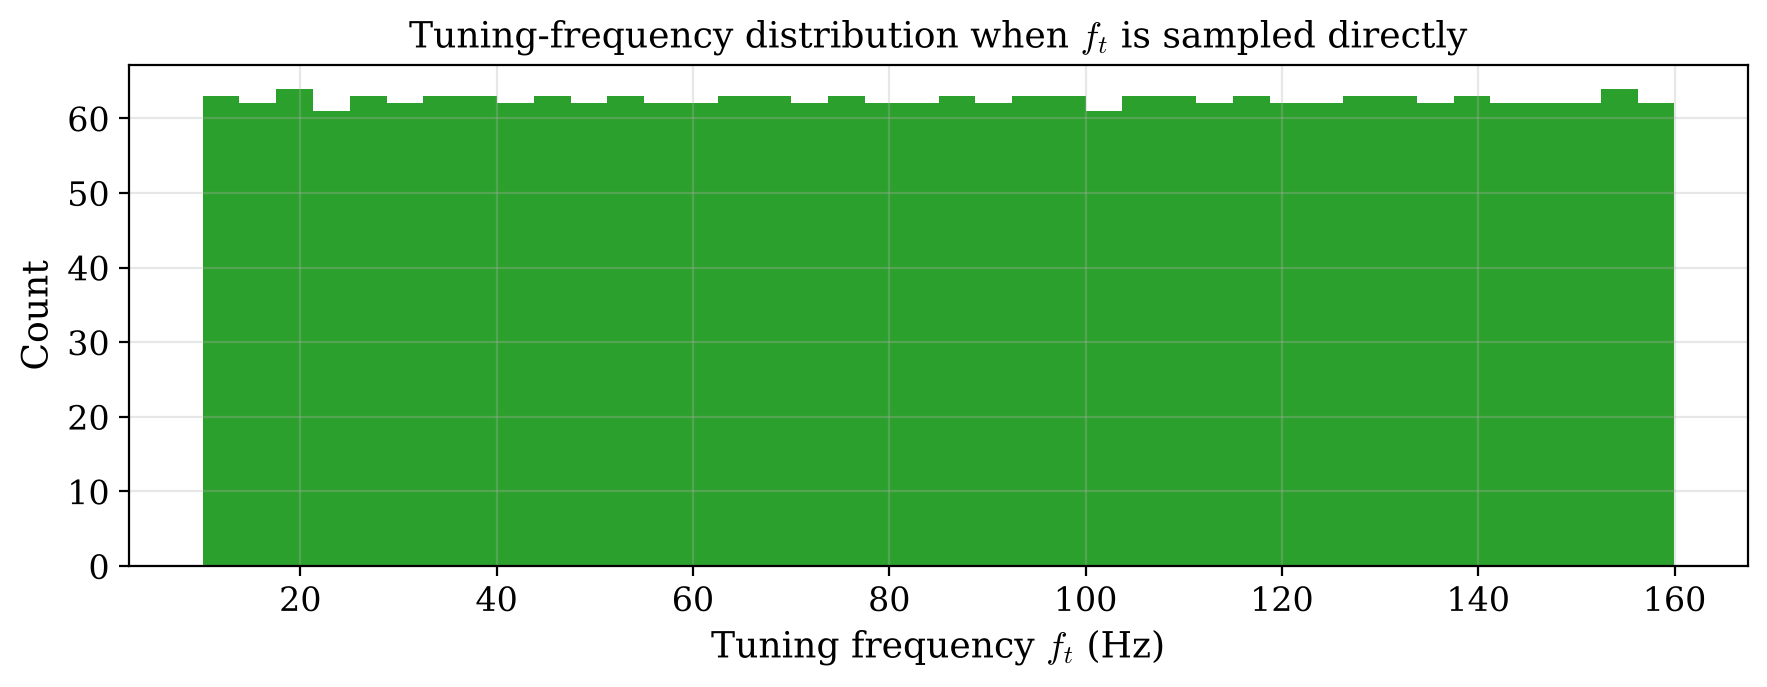
\includegraphics[width=0.95\textwidth]{Bilder/sampling_direct_ft.png}
\caption[Tuning frequency distribution when sampled directly]{Tuning-frequency distribution when $f_t$ is itself one of the sampled variables: close to uniform across the target band.}
\label{fig:sampling-direct}
\end{figure}

\begin{figure}[h]
\centering
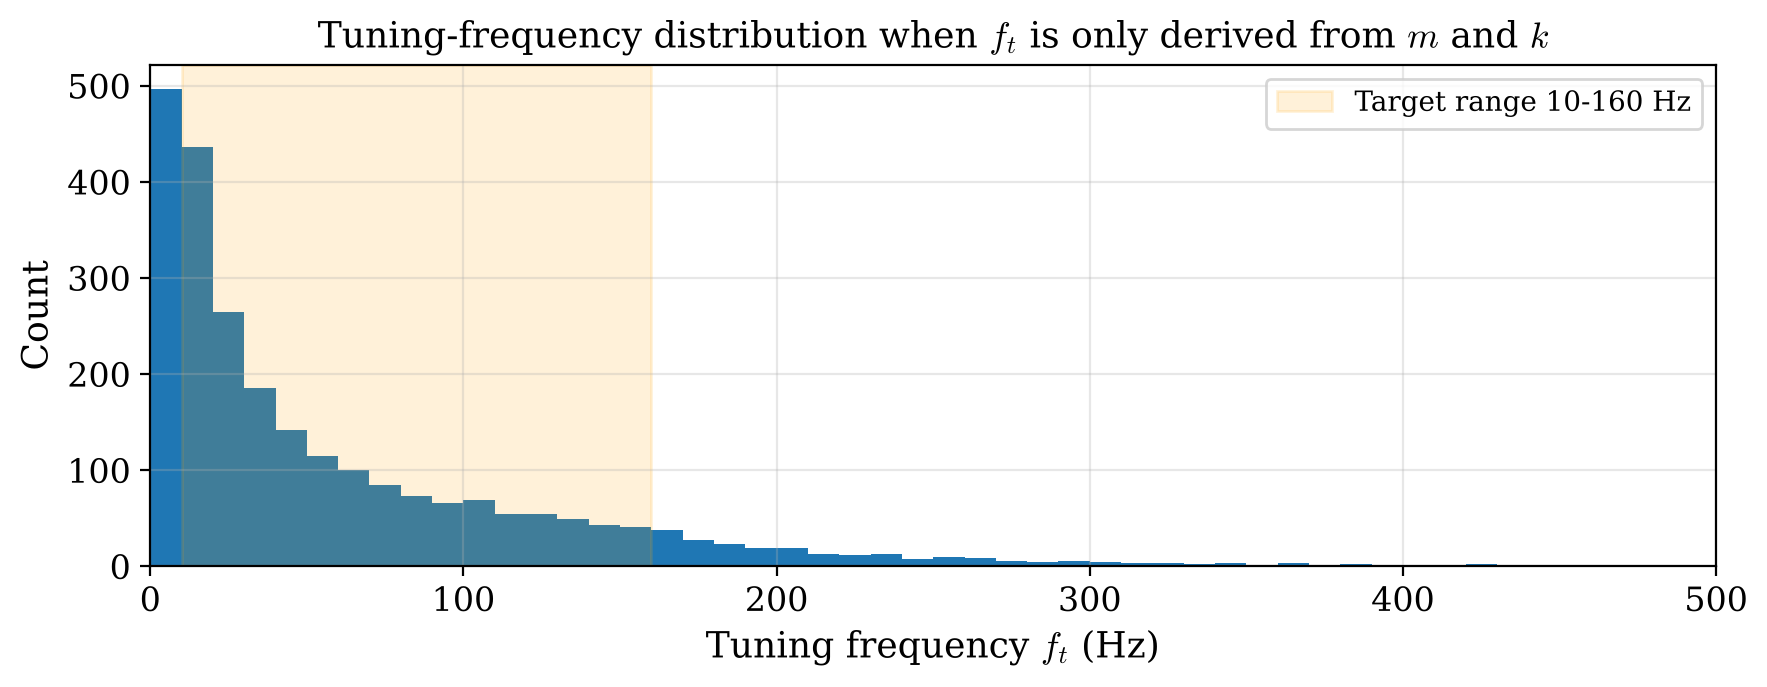
\includegraphics[width=0.95\textwidth]{Bilder/sampling_bias_mk.png}
\caption[Sampling bias when the tuning frequency is only derived]{Tuning-frequency distribution when mass and stiffness are sampled directly instead and the tuning frequency is only derived from them: the shaded target band is covered very unevenly.}
\label{fig:sampling-bias}
\end{figure}

For every sampled configuration, a modal physics solver computes the equivalent radiated power (ERP) spectrum at 301 frequencies between 10 and 160\,Hz. The plate's vibration is written as a sum of its own mode shapes plus the added resonator degrees of freedom, and the resulting linear system is solved at every frequency; the resonator degrees of freedom are then eliminated analytically so that only a small system, the size of the number of resonators, needs to be solved per frequency, which keeps dataset generation practical even for a hundred thousand configurations. Three datasets are used in this thesis, all solved with 18 plate modes ($6\times3$): two forward datasets of 100{,}000 configurations each, one with two and one with three resonators, in the five-variable design space described above, and an earlier two-resonator dataset of 200{,}000 configurations with four bounded design variables per resonator and a fixed damping coefficient, used for the invertible models (Section~\ref{sec:idon}). Figure~\ref{fig:erp-distribution} shows the resulting spread of ERP spectra across each of them, at every one of the 301 frequency points. The three datasets look alike: the ERP values average 84.0, 83.5 and 84.2\,dB with standard deviations of 9.8, 9.5 and 10.1\,dB, the median spectrum rises with frequency and shows clear peaks near the bare plate's own natural frequencies (dashed lines), and individual configurations vary widely around it, which is exactly the variety a surrogate model needs to learn from. The three-resonator dataset has a slightly lower mean and a smaller maximum than the two-resonator dataset, plausibly because a third resonator takes up more of the plate's vibration energy.

\begin{figure}[h]
\centering
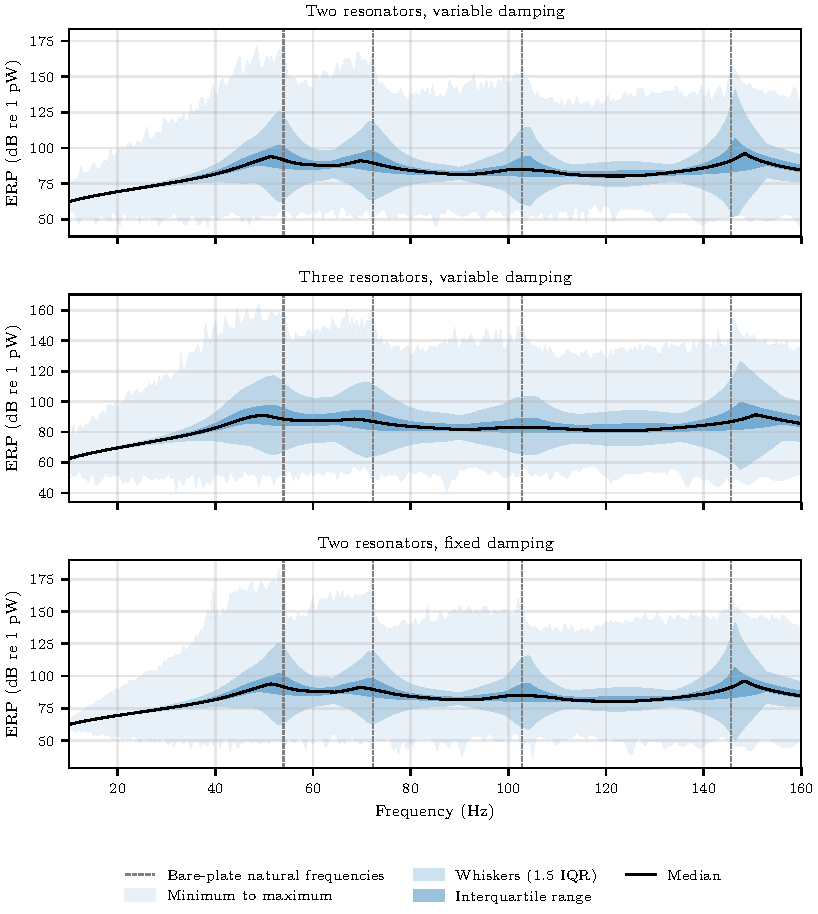
\includegraphics[max width=\textwidth]{Bilder/erp_distribution_datasets.pdf}
\caption[ERP distribution across the 301 frequency points]{Distribution of the ERP spectrum across all configurations of the three datasets, at each of the 301 frequency points: two resonators with sampled damping (100{,}000 configurations), three resonators with sampled damping (100{,}000) and two resonators with fixed damping (200{,}000). The shaded bands show the full range, the whiskers (1.5 times the interquartile range), the interquartile range and the median.}
\label{fig:erp-distribution}
\end{figure}

What does the biased sampling of Figure~\ref{fig:sampling-bias} actually do to the data a model would learn from? To check this directly, 2{,}000 configurations were sampled with mass and stiffness drawn directly and the tuning frequency derived, the same scheme as Figure~\ref{fig:sampling-bias}, and solved with the same solver. Figure~\ref{fig:erp-distribution-biased} shows the resulting ERP distribution, in the same style as the panels of Figure~\ref{fig:erp-distribution}. The overall spread of ERP values across this biased dataset is not noticeably smaller than the well-sampled one, but its median keeps sharp, tall peaks at the bare plate's natural frequencies (up to about 109\,dB, against about 96\,dB in the well-sampled dataset), because most resonators are tuned at low frequencies and hardly act on the plate's own resonances; what changes is where the data is concentrated. Because the derived tuning frequencies pile up at the low end of the band (Figure~\ref{fig:sampling-bias}), most of the training configurations are easy, repetitive examples from the same low-frequency region, while the higher part of the band is covered by only a handful of configurations. A model trained on this would see a low average test error, since most test examples fall in the dense, easy region it has seen many times, while being unreliable on the sparse, under-represented region. The average error alone would look good without the model having learned to generalise across the whole band; this is why this thesis reports accuracy at the resonance peaks separately from the overall accuracy, and why every design variable is sampled directly and evenly in the first place.

\begin{figure}[h]
\centering
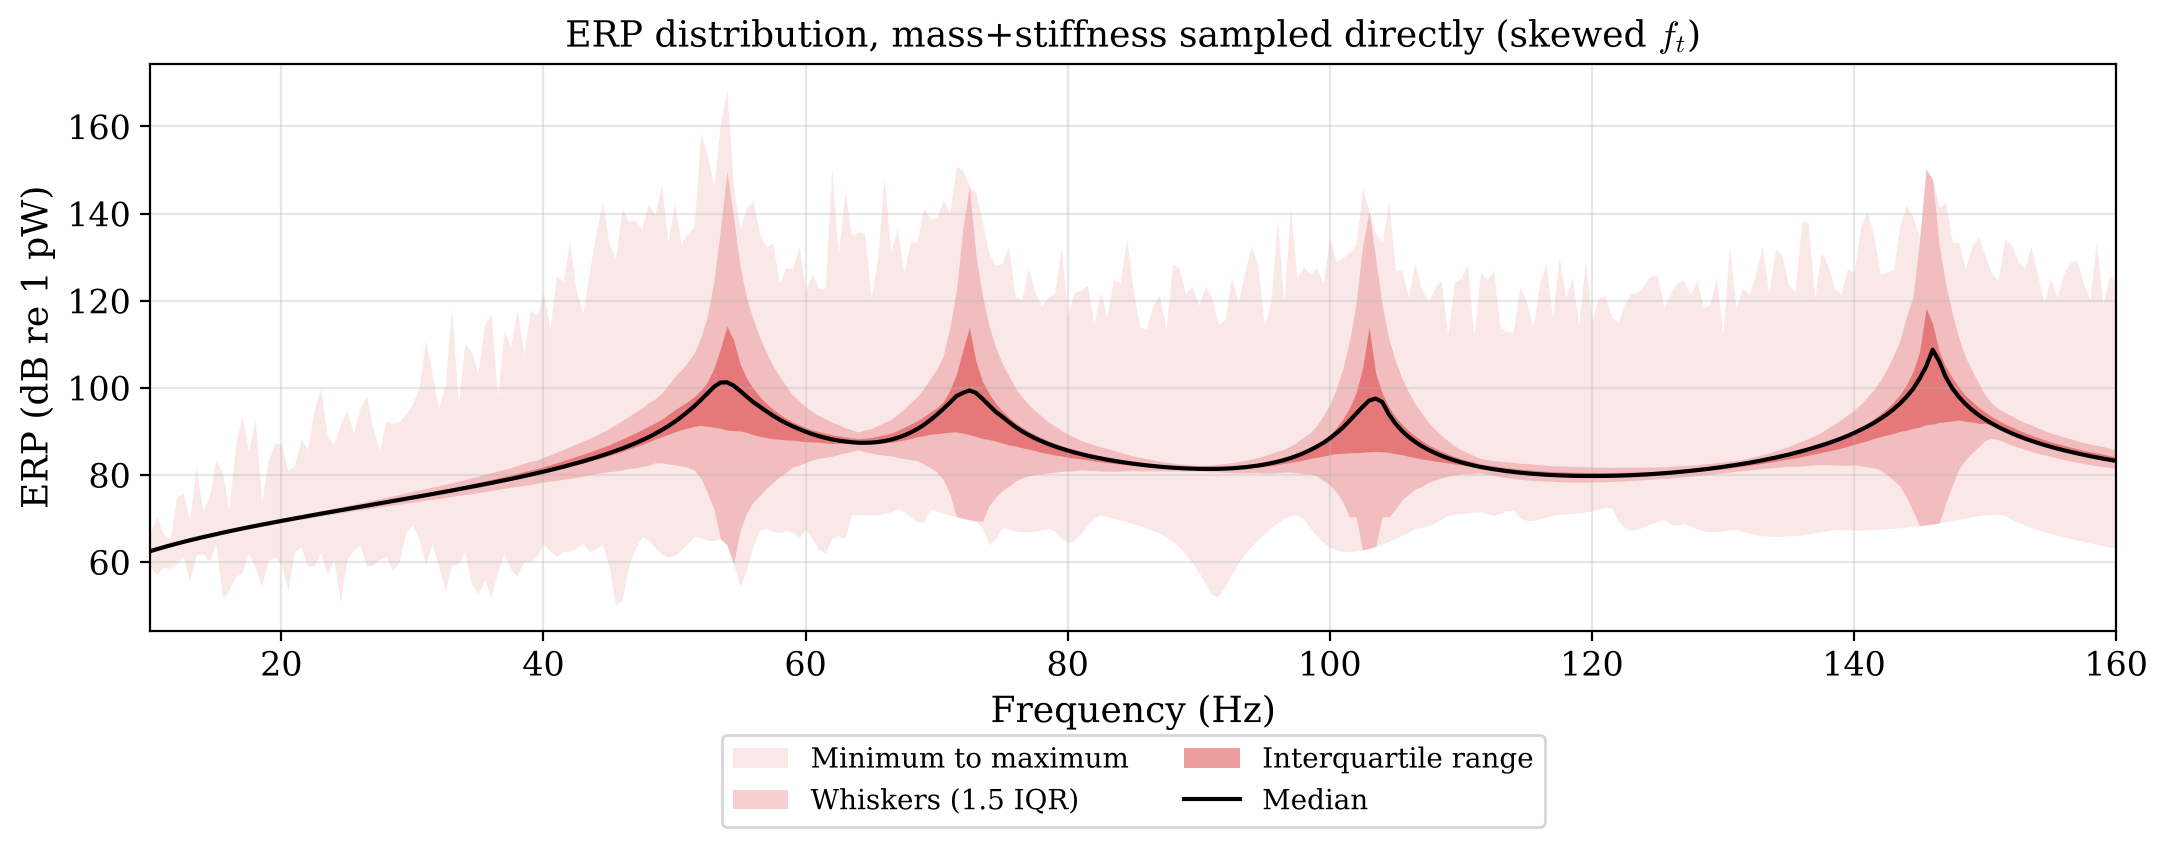
\includegraphics[width=0.95\textwidth]{Bilder/erp_distribution_biased.png}
\caption[ERP distribution under biased sampling]{ERP distribution of 2{,}000 configurations sampled the same way as Figure~\ref{fig:sampling-bias} (mass and stiffness sampled directly, tuning frequency derived and skewed low). Compare with Figure~\ref{fig:erp-distribution}.}
\label{fig:erp-distribution-biased}
\end{figure}

The dataset is split 80/10/10 into training, validation and test configurations, and every model in this thesis is trained and compared on the same split.

\section{Forward Architectures}
\label{sec:forward-architectures}

A forward architecture takes a resonator design and a query frequency as input and predicts the ERP value at that frequency. Nine of the ten architectures compared in this thesis share the same building blocks around a different core, shown in Figure~\ref{fig:forward-block}; only the plain baseline NN, described below, works on the raw design and frequency without them. The shared blocks are a resonator encoder that turns the set of resonators into a fixed-size description, since the plate's response does not depend on the order the resonators are listed in; a resonance query block that gives the network the distance between the query frequency and each resonator's tuning frequency; and a frequency encoder for the query frequency itself. The only part that changes between these architectures is the core architecture block; a shared decoder turns its output into the predicted ERP value.

\begin{figure}[h]
\centering
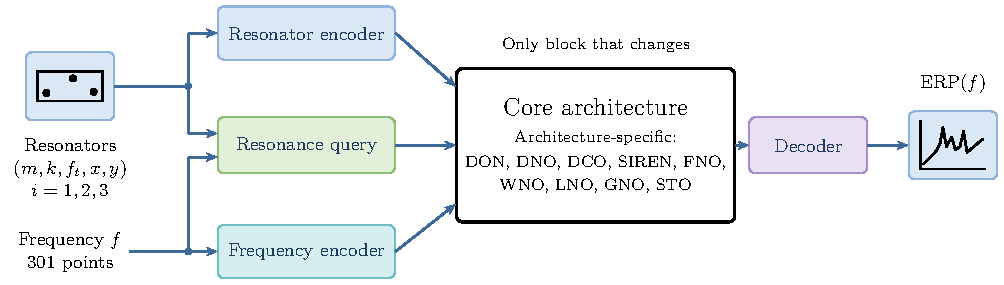
\includegraphics[max width=\textwidth]{Bilder/block_forward_architecture.pdf}
\caption[Forward architecture block diagram]{Shared structure of the nine encoder-based forward architectures: only the core architecture block changes between them. The baseline NN has no encoder blocks.}
\label{fig:forward-block}
\end{figure}

The ten forward architectures are, in short:

\begin{itemize}
  \item \textbf{DON} (DeepONet): a branch network encodes the design, a trunk network encodes the frequency, and the two are combined into a spectrum through a shared, orthonormal frequency basis \parencite{lu2021deeponet}.
  \item \textbf{DNO} and \textbf{DCO}: two architectures developed for this thesis rather than taken from a specific paper, which build on a stack of residual blocks \parencite{he2016resnet} in two different ways: DNO modulates each block with the resonator encoding through feature-wise linear modulation \parencite{perez2018film}, DCO concatenates the encodings of the resonators and of the frequency before the blocks.
  \item \textbf{SIREN}: a network of sine-activated layers, which tends to fit smooth oscillatory signals well \parencite{sitzmann2020siren}.
  \item \textbf{FNO} (Fourier neural operator): processes the frequency axis with learned convolutions in the Fourier domain \parencite{li2021fno}.
  \item \textbf{WNO} (wavelet neural operator): the same idea with a wavelet transform instead, which can better localise sharp resonance peaks \parencite{tripura2022wno}.
  \item \textbf{LNO} (Laplace neural operator): represents the spectrum through a small set of learned poles and residues, a natural fit for a system built from resonances \parencite{cao2023lno}.
  \item \textbf{GNO} (graph neural operator): treats the resonators as nodes of a graph and lets them exchange messages before predicting the spectrum \parencite{li2020graphno,gilmer2017mpnn}.
  \item \textbf{STO} (Set Transformer operator): uses attention between the resonators and the query frequency instead of message passing \parencite{lee2019settransformer,vaswani2017attention}.
  \item \textbf{NN}: a plain feed-forward network on the raw design and frequency (a multilayer perceptron, a universal approximator of continuous functions \parencite{hornik1989approximation}), used as a simple baseline.
\end{itemize}

Every architecture is sized to about 145{,}000 parameters (between 143{,}000 and 156{,}000 for the two forward datasets), so that differences in accuracy reflect the architecture itself rather than one model simply being larger than another.

\section{Invertible Architectures and Generative Design}

An invertible architecture is built the same way as a forward one, except that its core is made of blocks that can be run backward as well as forward. Running it forward predicts a spectrum from a design, exactly like the forward architectures above; running the same weights backward turns a target spectrum into a proposed design. Figure~\ref{fig:operators-overview} summarises the difference between the three kinds of model used in this thesis: a forward operator maps one design to one spectrum; an inverse-only operator would map one spectrum to many possible designs; an invertible operator does both with the same weights, so the two directions stay consistent with each other.

\begin{figure}[h]
\centering
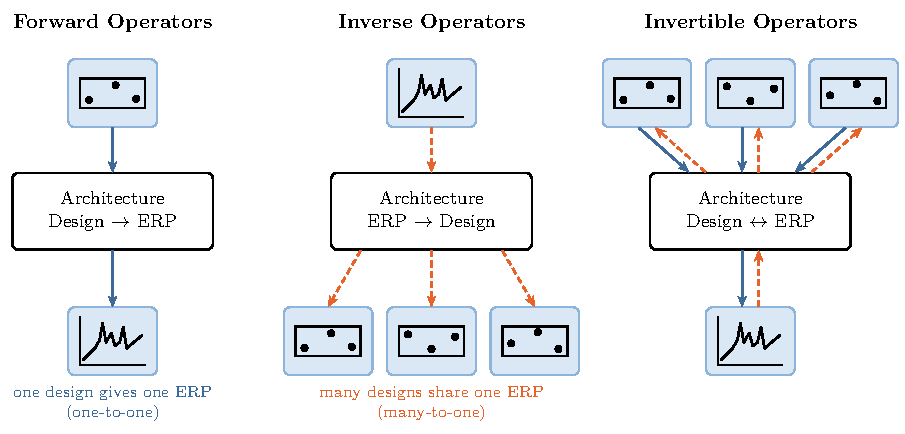
\includegraphics[max width=\textwidth]{Bilder/block_operators_overview.pdf}
\caption[Forward, inverse and invertible operators]{Forward operators map one design to one spectrum (one-to-one); the inverse direction maps one spectrum to many possible designs (many-to-one); an invertible operator combines both directions in one set of weights.}
\label{fig:operators-overview}
\end{figure}

This two-direction property is what makes generative design possible: given a target ERP spectrum, for example one with a deep notch at a frequency an engineer wants quiet, the inverse direction proposes one or several resonator designs that should produce it, without needing a separate search or optimisation loop. A proposed design can then be checked by running it back through the forward direction, or through the physics solver directly, and its robustness to manufacturing tolerances can be checked with the Monte Carlo procedure described in Chapter~\ref{ch:theory}. This thesis builds seven invertible architectures: an invertible DeepONet (iDON), described in Section~\ref{sec:idon}, and an iFNO family of six more architectures, described in Section~\ref{sec:ifno}.

\subsection{iDON}
\label{sec:idon}

iDON \parencite{kaltenbach2023invertible} keeps the DeepONet idea of a branch network for the design and a trunk network for the frequency, but makes the branch itself exactly invertible, shown in Figure~\ref{fig:idon-block}. The branch is a RealNVP coupling flow \parencite{dinh2017realnvp}: it maps the design $a$ to a vector of $Q$ coefficients $b$, and because every RealNVP layer is a coupling block of the kind described in Chapter~\ref{ch:theory}, this map can be run backward to recover $a$ from $b$ exactly, with no approximation. The trunk is an ordinary network that maps the frequency to an orthonormal basis $\Psi(f)$, shared by both directions. In this thesis the branch consists of ten RealNVP coupling layers with 256 hidden units each, and the trunk applies four hidden layers of 256 units to the frequency and to its sine and cosine features at 32 harmonics. The forward direction predicts the spectrum as $\mathrm{ERP}(f) = \Psi(f)\,b + \psi_0$; the inverse direction projects a target spectrum onto the same basis, $b^\ast = \Psi^T(y - \psi_0)/F$, and runs the branch backward to recover a design from $b^\ast$.

\begin{figure}[h]
\centering
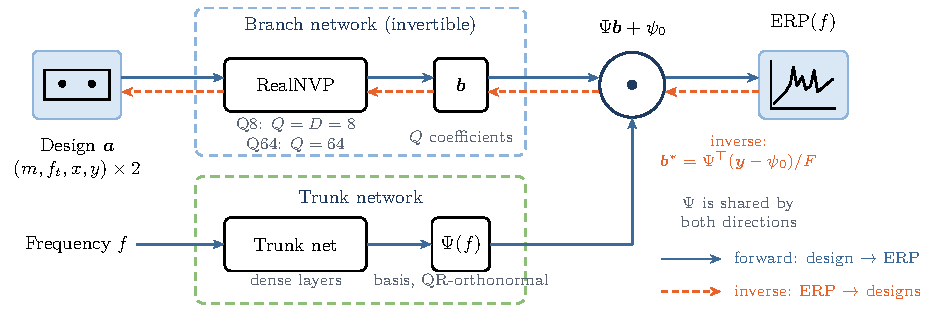
\includegraphics[max width=\textwidth]{Bilder/block_idon_architecture.pdf}
\caption[iDON block diagram]{iDON: an invertible RealNVP branch network maps a design to $Q$ coefficients and back; an ordinary trunk network supplies a shared, orthonormal frequency basis.}
\label{fig:idon-block}
\end{figure}

The numbers reported for iDON and the iFNO family in this section and in Chapter~\ref{ch:results} come from an earlier, larger two-resonator dataset of 200{,}000 configurations, built before the damping ratio became a sampled design variable: each resonator is described by four bounded numbers, mass, tuning frequency and position, with a fixed damping coefficient. The architectures and the invertibility mechanism are identical to the ones described here; only this particular dataset predates the five-variable design space of Section~\ref{sec:design-space}.

How many coefficients $Q$ should the branch produce? The most direct choice is $Q = D$, the number of numbers in the design itself (so a two-resonator design with four bounded numbers each gives $D=8$); this thesis calls that configuration Q8. A strictly invertible branch with $Q=D$ is bijective, but it also means the basis $\Psi(f)$ has only as many degrees of freedom as the design, which turned out to be too few to represent the ERP spectrum well: on the two-resonator, 200{,}000-configuration dataset used for the invertible models, Q8 reaches only 6.05\,dB forward RMSE and recovers the tuning frequency with a Pearson correlation of 0.81 (Table~\ref{tab:idon-q}). The fix used in this thesis, and in \textcite{kaltenbach2023invertible}, is to pad the branch to a larger $Q$, for example $Q=64$ (Q64): the branch still outputs a vector of length $Q$, but only the first $D$ numbers correspond to the physical design, and the remaining $Q-D$ are extra, padded latent values $z$ that have no physical meaning. With more coefficients to work with, the trunk can represent the spectrum far more accurately: Q64 reaches 2.67\,dB forward RMSE, and recovers the tuning frequency with a Pearson correlation of 0.87, a clear improvement over Q8 on every metric checked in this thesis. The padding only helps if the extra latent values stay small and uninformative, otherwise the model could hide part of the true design signal in them where the inverse direction cannot see it; this is enforced by adding a padding loss term, $\mathcal L_\text{pad} = \mathrm{Huber}(\hat z, 0)$ \parencite{huber1964robust}, that pulls the recovered padded values toward zero during training. Every result for iDON reported in Chapter~\ref{ch:results} uses the padded Q64 configuration.

\subsection{iFNO and the Rest of the Family}
\label{sec:ifno}

The other six invertible architectures, iDNO, iDCO, iFNO, iLNO, iGNO and iSTO, share one common pipeline instead of each being built from scratch, shown in Figure~\ref{fig:ifno-block}. A design is lifted to a latent representation by a block $P$, together with the query frequency; the latent representation passes through a coupling stack, the same kind of invertible block described in Chapter~\ref{ch:theory}, which uses the same weights in both directions; a readout block $Q$ turns the latent representation into the predicted ERP. The inverse direction mirrors this exactly: a lift $P'$ turns a target spectrum into a latent representation, the same coupling stack runs backward, and a readout $Q'$ turns the result into a proposed design.

\begin{figure}[h]
\centering
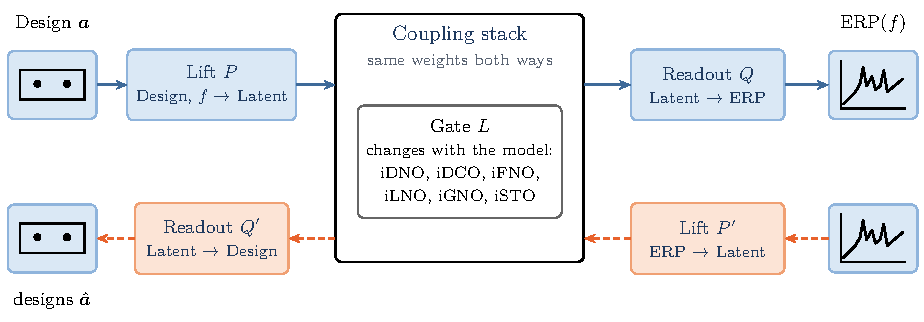
\includegraphics[max width=\textwidth]{Bilder/block_invertible_operator_architecture.pdf}
\caption[iFNO family block diagram]{Shared pipeline of the iFNO family. Only the gate $L$ inside the coupling stack changes between iDNO, iDCO, iFNO, iLNO, iGNO and iSTO; the lifts, readouts and the rest of the coupling stack are the same.}
\label{fig:ifno-block}
\end{figure}

Only the coupling stack is an exact bijection between latent tensors; the lifts and readouts are ordinary, learned (and therefore lossy) networks, so the pipeline as a whole is a bidirectional model with an invertible core rather than an exactly invertible map from design to spectrum. What distinguishes the six family members from one another is only the gate $L$ inside each coupling block: iDNO uses a residual-block gate conditioned on a learned embedding of the frequency, matching DNO \parencite{perez2018film}; iDCO uses a residual-block gate matching DCO \parencite{he2016resnet}; iFNO uses a spectral convolution gate, the invertible counterpart of the FNO core \parencite{li2021fno}; iLNO uses a learned pole-residue gate matching LNO \parencite{cao2023lno}; iGNO uses a graph message-passing gate matching GNO \parencite{li2020graphno}; and iSTO uses a frequency-mixing gate in place of STO's attention \parencite{lee2019settransformer}. This mirrors how the nine encoder-based forward architectures in Section~\ref{sec:forward-architectures} share an encoder and a decoder and differ only in their core block: here, the lift, coupling stack and readout stay fixed, and only the gate inside the coupling stack is architecture-specific. Training follows the three-stage recipe of \textcite{long2025invertiblefno}, detailed in Section~\ref{sec:training}: first the invertible core and the lifts and readouts, then a $\beta$-variational step \parencite{kingma2014vae,higgins2017betavae} that turns a single estimated design into a small family of plausible designs (needed because, as Chapter~\ref{ch:theory} showed, the inverse is rarely unique), then all parts trained together.

\section{Training}
\label{sec:training}

All models are trained on the 80/10/10 split described in Section~\ref{sec:design-space}, with the ERP and the design variables normalised by the statistics of the training split, and the weights of the epoch with the lowest validation loss are kept.

The ten forward architectures are trained for 200 epochs with a batch size of 128 using AdamW \parencite{loshchilov2019adamw} with a weight decay of $10^{-4}$, a learning rate of $5\times10^{-4}$ ($2\times10^{-4}$ for SIREN) that decays along a cosine schedule to $10^{-6}$, and gradient-norm clipping at 5. The loss is not the plain mean squared error. It adds the mean squared error of the spectrum's slope between neighbouring frequencies, with weight 0.5, and the squared error at the resonance peaks of the target spectrum, with weight 0.05, so that the narrow peaks, which carry most of the acoustic information, are not neglected. NN has no permutation-invariant encoder, so the order of the resonators is shuffled in every batch to keep it from depending on the order.

The six architectures of the iFNO family are trained in three stages, as described in Section~\ref{sec:ifno}, with up to 100, 25 and 50 epochs, learning rates of $5\times10^{-4}$, $10^{-3}$ and $3\times10^{-4}$ with a cosine decay, a batch size of 128 and gradient-norm clipping at 5. The weight of the variational term is $\beta = 0.05$, reached after a warm-up over the first 8 epochs of the second stage \parencite{higgins2017betavae}, and the cycle-consistency and alignment terms of the first and third stage have weight 0.1. A stage ends early if its validation loss has not improved for 10 epochs. This happened in the first stage of iFNO (after 65 epochs) and iGNO (71 epochs) and in the third stage of iFNO (after 25 epochs); iLNO and iSTO ran the full 100, 25 and 50 epochs. iDNO and iDCO were trained with a shorter schedule of 50, 15 and 15 epochs, so their results in Chapter~\ref{ch:results} may improve with the full schedule.

iDON is trained for 150 epochs with a learning rate of $5\times10^{-4}$. Its loss is the sum of the forward spectrum loss above, whose peak term is only switched on in the last 20\,\% of the epochs, a Huber loss \parencite{huber1964robust} on the design recovered from the true spectrum, whose weight rises from zero to one over the first 10 epochs, and the padding term of Section~\ref{sec:idon} with weight 0.1. The Q8 variant stopped early: its validation loss stopped improving after epoch 37, and training ended after 50 of the 150 planned epochs, whereas Q64 ran all 150 epochs.

The invertible operators were not all trained with the same parameters and epochs: the training was carried out on a CPU, with only limited GPU session time available, so the learning rates, the number of epochs and the stage schedules were chosen to fit the available compute and differ between models, as described above. Results from further training runs with other settings, if they become available, will be published in the GitHub repository (and the LRZ Sync\&Share folder) given in Appendix~B.

\section{A Single, Reproducible Pipeline}

The physics solver, the dataset generation, the ten forward architectures and the seven invertible architectures described above are all implemented in one Python script. Running it solves resonator configurations, builds a dataset, and trains and evaluates whichever models are selected, without any other setup. This was a deliberate choice: keeping the whole pipeline in one place, with one consistent way of encoding a design and one consistent training loop, makes the results in this thesis straightforward for another person to reproduce from the dataset variables and architecture descriptions given above.
